\documentclass[fontsize=12pt, paper=a4, headinclude, twoside=false, parskip=half+, pagesize=auto, numbers=noenddot, open=right, toc=listof, toc=bibliography]{scrreprt}
% PDF-Kompression
\pdfminorversion=5
\pdfobjcompresslevel=1
% Allgemeines
\usepackage[automark]{scrpage2} % Kopf- und Fußzeilen
\usepackage{amsmath,marvosym} % Mathesachen
\usepackage[T1]{fontenc} % Ligaturen, richtige Umlaute im PDF
\usepackage[utf8]{inputenc}% UTF8-Kodierung für Umlaute usw
% Schriften
\usepackage{mathpazo} % Palatino für Mathemodus
%\usepackage{mathpazo,tgpagella} % auch sehr schöne Schriften
\usepackage{setspace} % Zeilenabstand
\onehalfspacing % 1,5 Zeilen
% Schriften-Größen
\setkomafont{chapter}{\Huge\rmfamily} % Überschrift der Ebene
\setkomafont{section}{\Large\rmfamily}
\setkomafont{subsection}{\large\rmfamily}
\setkomafont{subsubsection}{\large\rmfamily}
\setkomafont{chapterentry}{\large\rmfamily} % Überschrift der Ebene in Inhaltsverzeichnis
\setkomafont{descriptionlabel}{\bfseries\rmfamily} % für description Umgebungen
\setkomafont{captionlabel}{\small\bfseries}
\setkomafont{caption}{\small}
% Sprache: Deutsch
\usepackage[ngerman]{babel} % Silbentrennung
% PDF
\usepackage[ngerman,pdfauthor={Martin Bretschneider},  pdfauthor={Martin Bretschneider}, pdftitle={Vorlage für LaTeX}, breaklinks=true,baseurl={http://www.bretschneidernet.de/tips/thesislatex.html}]{hyperref}
\usepackage[final]{microtype} % mikrotypographische Optimierungen
\usepackage{url} % ermögliche Links (URLs)
\usepackage{pdflscape} % einzelne Seiten drehen können
% Tabellen
\usepackage{multirow} % Tabellen-Zellen über mehrere Zeilen
\usepackage{multicol} % mehre Spalten auf eine Seite
\usepackage{tabularx} % Für Tabellen mit vorgegeben Größen
\usepackage{longtable} % Tabellen über mehrere Seiten
\usepackage{array}
%  Bibliographie
\usepackage{bibgerm} % Umlaute in BibTeX
% Tabellen
\usepackage{multirow} % Tabellen-Zellen über mehrere Zeilen
\usepackage{multicol} % mehre Spalten auf eine Seite
\usepackage{tabularx} % Für Tabellen mit vorgegeben Größen
\usepackage{array}
\usepackage{float}
% Bilder
\usepackage{graphicx} % Bilder
\usepackage{color} % Farben
\graphicspath{{images/}}
\DeclareGraphicsExtensions{.pdf,.png,.jpg} % bevorzuge pdf-Dateien
\usepackage{subcaption}  % mehrere Abbildungen nebeneinander/übereinander

\usepackage[all]{hypcap} % Beim Klicken auf Links zum Bild und nicht zu Caption gehen
% Bildunterschrift
\setcapindent{0em} % kein Einrücken der Caption von Figures und Tabellen
\setcapwidth{0.9\textwidth} % Breite der Caption nur 90% der Textbreite, damit sie sich vom restlichen Text abhebt
\setlength{\abovecaptionskip}{0.2cm} % Abstand der zwischen Bild- und Bildunterschrift
% Quellcode
\usepackage{listings} % für Formatierung in Quelltexten
\definecolor{grau}{gray}{0.25}
\lstset{
	extendedchars=true,
	basicstyle=\tiny\ttfamily,
	%basicstyle=\footnotesize\ttfamily,
	tabsize=2,
	keywordstyle=\textbf,
	commentstyle=\color{grau},
	stringstyle=\textit,
	numbers=left,
	numberstyle=\tiny,
	% für schönen Zeilenumbruch
	breakautoindent  = true,
	breakindent      = 2em,
	breaklines       = true,
	postbreak        = ,
	prebreak         = \raisebox{-.8ex}[0ex][0ex]{\Righttorque},
}
% linksbündige Fußboten
\deffootnote{1.5em}{1em}{\makebox[1.5em][l]{\thefootnotemark}}

\typearea{14} % typearea berechnet einen sinnvollen Satzspiegel (das heißt die Seitenränder) siehe auch http://www.ctan.org/pkg/typearea. Diese Berechnung befindet sich am Schluss, damit die Einstellungen oben berücksichtigt werden

\usepackage{scrhack} % Vermeidung einer Warnung


% Eigene Befehle %%%%%%%%%%%%%%%%%%%%%%%%%%%%%%%%%%%%%%%%%%%%%%%%%5
% Matrix
\newcommand{\mat}[1]{
      {\textbf{#1}}
}
\newcommand{\todo}[1]{
      {\colorbox{red}{ TODO: #1 }}
}
\newcommand{\todotext}[1]{
      {\color{red} TODO: #1} \normalfont
}
\newcommand{\info}[1]{
      {\colorbox{blue}{ (INFO: #1)}}
}
% Hinweis auf Programme in Datei
\newcommand{\datei}[1]{
      {\ttfamily{#1}}
}
\newcommand{\code}[1]{
      {\ttfamily{#1}}
}
% bild mit defnierter Breite einfügen
\newcommand{\bild}[4]{
  \begin{figure}[!hbt]
    \centering
      \vspace{1ex}
      \includegraphics[width=#2]{images/#1}
      \caption[#4]{\label{img.#1} #3}
    \vspace{1ex}
  \end{figure}
}
% bild mit eigener Breite
\newcommand{\bilda}[3]{
  \begin{figure}[!hbt]
    \centering
      \vspace{1ex}
      \includegraphics{images/#1}
      \caption[#3]{\label{img.#1} #2}
      \vspace{1ex}
  \end{figure}
}


% Bild todo
\newcommand{\bildt}[2]{
  \begin{figure}[!hbt]
    \begin{center}
      \vspace{2ex}
	      \includegraphics[width=6cm]{images/todobild}
      %\caption{\label{#1} \color{red}{ TODO: #2}}
      \caption{\label{#1} \todotext{#2}}
      %{\caption{\label{#1} {\todo{#2}}}}
      \vspace{2ex}
    \end{center}
  \end{figure}
} % Importiere die Einstellungen aus der Präambel
% hier beginnt der eigentliche Inhalt
\begin{document}
\pagenumbering{Roman} % Seitenummerierung mit großen römischen Zahlen 
\pagestyle{empty} % kein Kopf- oder Fußzeilen auf den ersten Seiten

% Titelseite
\clearscrheadings\clearscrplain
\begin{center}
\begin{Huge}
Fachhochschule Wedel\\
\vspace{3mm}
\end{Huge}
{\Large Studiengang Medieninformatik}\\

\vspace{20mm}
\begin{Large}
Eine Einführung in die prozedurale Landschaftsgenerierung\\
\end{Large}
\vspace{8mm}
Seminararbeit\\
\vspace{0.4cm}
\vspace{2 cm}
Tjark Smalla \\
Matrikel-Nummer 100554\\
\vspace{8cm}
\begin{tabular}{rl}
{\bfseries Betreuer} & Prof. Bohn\\
\end{tabular}

\end{center}
\clearpage


\pagestyle{useheadings} % normale Kopf- und Fußzeilen für den Rest

\tableofcontents % erstelle hier das Inhaltsverzeichnis
\listoffigures % erstelle hier das Abbildungsverzeichnis
\listoftables % erstelle hier das Tabellenverzeichnis

\addchap{Symbolverzeichnis}\label{s.sym} % vergebe für das Symbolverzeichnis keine Kapitelnummer
\section*{Allgemeine Symbole}\label{s.sym.alg}
\begin{flushleft}\begin{tabularx}{\textwidth}{l|X}
Symbol & Bedeutung\\\hline
$a$ & der Skalar $a$ \\
$\vec{x}$ & der Vektor $\vec{x}$\\
$\mat{A}$ & die Matrix $\mat{A}$\\
\end{tabularx}\end{flushleft}




% richtiger Inhalt
\chapter{Einleitung}
\pagenumbering{arabic} % ab jetzt die normale arabische Nummerierung

Während die künstliche Erzeugung von Landschaften\footnote{Landschafts-Synthese} in der Computergrafik schon seit den 80gern ein Thema ist, beschäftigte sich auch Hersteller von Computerspielen immer wieder mit dieser Technik. Insbesondere in den letzten 10 Jahren begannen immer mehr Entwickler diese Technik anzuwenden.

Die prozedurale Generierung ihrer Landschaften bietet ihnen viele Vorteile. 
Durch die mittlerweile sehr großen Spielwelten ist es nicht unüblich bis zu 300 Leute über 2 Jahre an nur einem großen Projekt zu beschäftigen. Ein großer Teil dieser Zeit wird in die Ausgestaltung der Spielwelt gesteckt. Prozedurale Techniken erlauben es ihnen realistische Spielwelten zu erschaffen die nahezu unendlich groß sind.
Als bekanntestes Beispiel ist hier sicherlich das Spiel Minecraft vom Studio Mojang zu nennen, welches einen Großteil seiner Faszination aus der komplett prozedural erzeugten veränderbaren Landschaft zieht.

Im folgenden werden 3 bewährte Algorithmen zur Erzeugung von Landschaften vorgestellt und daraufhin untersucht, in wie weit sie zur Speicherung einer nahezu unendlich großen Landschaft wie in Minecraft geeignet sind.

Zuerst wird der \emph{Diamond-Square} Algorithmus\cite{DiamondSquare} vorgestellt, welchen man verallgemeinert auch als einen Polygon unterteilungs Algorithmus bezeichnen kann. Danach wird kurz die \emph{Spektalsynthese} mit der Fourier-Methode erläutert bevor es eine Einführung in die Welt der Rauschfunktionen gibt. 
Neben der Synthese von Landschaften sind diese Algorithmen vielseitig einsetzbar. Insbesondere bei der bereits erwähnten Kategorie der Rauschfunktionen ist davon auszugehen, dass sie auch in proprietärer 3D-Software wie Computerspielen trotz ihres Alters noch als wichtiger Algorithmus genutzt werden. Dies liegt vor allem an ihrer Flexibilität sowie Skalierbarkeit in mehreren Dimensionen durch die auch Wolken, Feuer, Rauchverwirbelung und sogar Fell auf einer Oberfläche erfolgreich dargestellt wurden \cite{texturingAndModeling}\footnote{Wolken: Kapitel 9, Feuer(S,125) \& Rauchverwirbelung: Kapitel 12, Rauch, Wolken, Fell: S.297-302}.
Neben der Bewertung soll dabei insbesondere die Erklärung der Grundlagen dieser Algorithmen Zielsetzung sein. Zu diesem Zwecke wird neben der Erklärung im Unterkapitel \emph{"Der Algorithmus"} jedes Verfahren auf seine Erweiter- bzw. Anpassbarkeit(\emph{"Flexibilität"}) hin untersucht, bevor es eine abschließende \emph{"Bewertung im Rahmen der Fragestellung"}. In diesem letzten Schritt wird das Verfahren daraufhin untersucht, in wie weit es effektiv zur Speicherung und Auswertung einer nahezu unendlich großen Landschaft geeignet ist.

Der Diamond-Square Algorithmus sowie verschiedene Rauschfunktionen sind in dem dieser Arbeit beiliegendem Unity-Projekt in C\# bzw. HLSL\footnote{High Level Shading Language} implementiert und lassen sich durch Unity auf Windows, Unix und Mac OS basierten Betriebssystemen kompilieren.

\section{Datenstrukturen zur Landschaftsspeicherung: Höhenfelder vs. Voxel}
Landschaften werden in der Regel entweder in einem Höhenfeld oder in Voxeln gespeichert.
Der wesentliche Unterschied der beiden Techniken liegt in ihren Dimensionen. Das Höhenfeld speichert in einem ganzzahligen, zweidimensionalen Koordinatensystem zu jedem Punkt den dazugehörigen Höhenwert der Landschaft, während ein Voxel den Dichtewert eines Punktes in einem dreidimensionalem Koordinatensystem darstellt. Beide Datenstrukturen haben den Vorteil, dass sich die Position jedes Wertes in der Landschaft implizit aus der Position zu seinen Nachbarn bestimmen lässt. Eine zusätzliche Speicherung seiner Koordinate ist also nicht notwendig. Anders wäre es bei Polygonen, wo jeder Vertex eine Koordinate im Raum hat. Sie sind daher gut für Szenen mit viel leerraum geeignet, welcher allerdings in den hier vorgestellten Datenstrukturen zu unnötig gespeicherten Daten führe würde

\subsection{Höhenfelder}
Die meisten Algorithmen beziehen sich auf die Erzeugung von Landschaften mit Hilfe von Höhenfeldern. Dies ist vermutlich vor allem dem geschuldet, dass viele Algorithmen recht alt sind und sich Voxel basierte Verfahren aufgrund des Speicherplatzmangels nicht lohnten.
Auch wenn Höhenfelder bereits zu sehr realistischen Ergebnissen großer Landschaftsstriche führen, haben sie einen entscheidenden Nachteil. Da pro Punkt im Koordinatensystem nur ein Höhenwert gespeichert werden kann sind Höhlen oder Überhänge nicht möglich.

Aufgrund der vereinfachten Algorithmen und der großen Verbreitung wird sich im folgendem auf Höhenfelder beschränkt. Eine Erweiterung in die dritte Dimension ist mit dem Diamond-Square Algorithmus oder den Rauschfunktionen jedoch problemlos möglich.
Ein weiterer Vorteil von Höhenfeldern ist, dass sich durch die simple Verbindung nebeneinanderliegender Punkte sehr einfach ein Polygon erzeugen lässt, welches Hardwarebeschleunigt gerendert werden kann.

\begin{figure}
	\centering
	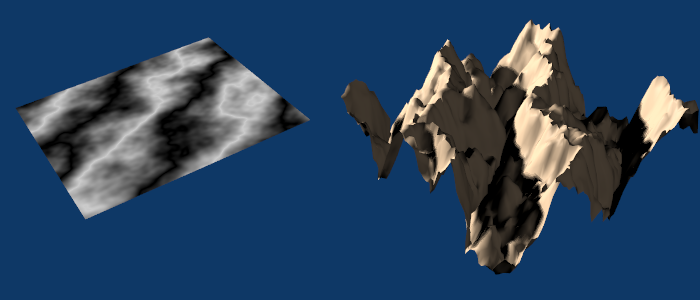
\includegraphics[width=\textwidth]{images/heightfield_rendered.png}
	\caption{Gegenüberstellung einer Heightfield als Textur(links) und der resultierenden Landschaft. Bildquelle: http://tinyurl.com/zu7gond}\label{img.heightfield}
\end{figure}

\subsection{Voxel}
Der Begriff Voxel leitet sich aus den Begriffen Volumen und Pixel ab.
Durch die Speicherung in einem dreidimensionalem Koordinatensystem wird nun auch die, bei den Höhenfeldern explizit gespeicherte, Höhe eines Punktes implizit gespeichert. Dies ermöglicht es eine weitere Information für jeden Punkt explizit zu speichern. In der Regel ist dies ein Dichtewert der es ermöglicht verschiedene Arten von Materialien oder die Opazität zu simulieren.

Um Voxel hardwarebeschleunigt zu rendern müssen auch diese in ein Polygon umgewandelt werden. Dies funktioniert normalerweise über Raycasting oder den Marching Cube Algorithmus.

\begin{figure}
	\centering
	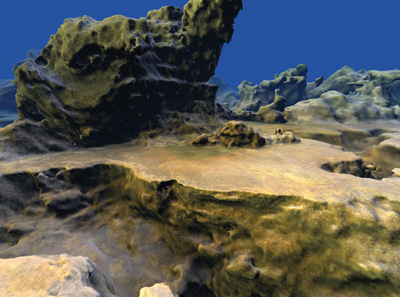
\includegraphics[width=\textwidth]{images/voxel_rendered.jpg}
	\caption{Gerenderte Voxellandschaft mit Überhängen erzeugt aus mehreren Rauschfunktionen. Bildquelle: http://tinyurl.com/jq8vta8}\label{img.heightfield}
\end{figure}

\section{Implizite vs. explizite Funktionen}
Alle hier vorgestellten Methoden lassen sich in 2 Gruppen einteilen: implizite und explizite Funktionen.
Während eine explizite Funktion alle Höhenpunkte auf einmal berechnet lässt sich die implizite Funktion für jeden Punkt, also jede Koordinate, isoliert auswerten. 

Durch die Unabhängigkeit der Berechnung für jeden einzelnen Punkt lassen sich implizite Algorithmen sehr effizient parralel auf einer GPU berechnen\footnote{Siehe Beispielimplementierung in einem Vertex-Shader}. Dies ermöglicht die Ausführung zur Laufzeit, während explizite Methoden in der Regel vor oder bei Programmstart einmalig berechnet werden und deren Ergebnisse in einer Textur gespeichert werden.
Dies hat den Vorteil, dass der Speicherbedarf enorm sinkt.

Ein Einsatzgebiet für diese Technik ist das Bump-Mapping bzw. Displacement Mapping bei der zusätzliche Höhenwerte auf ein Objekt durch Shading oder neue Vertices auf der Objektoberfläche hinzugefügt werden\cite{displacementNStuff}. Da moderne Echtzeitspiele immer mehr und immer größere Texturen verwenden steigt der Bedarf an Speicher enorm wenn für jede Textur noch eine Normal/Bump/Displacement Map gespeichert werden muss. Implizite Methoden erlauben es, anstatt der Texturen einige Parameter in Form von Floats und Integern zu speichern.
Auch eine Anpassung des Detailgrades ist zur Laufzeit ohne Probleme möglich, während bei der Detailgrad bei expliziten Methoden von der Auflösung der Textur abhängt\footnote{Diese Eigenschaften lassen sich zwar auch durch die Berechnung von expliziten Methoden zur Laufzeit erreichen, jedoch lassen diese sich wie erwähnt nicht effektiv durch die GPU beschleunigen wodurch die Berechnung innerhalb eines Frames unperformant ist.}.

Der Diamond-Square Algorithmus sowie die Spektralsynthese gehören zu der Gruppe der expliziten Algorithmen, während die Rauschfunktionen implizit auswertbar sind.

\chapter{Noise}\label{Noise}
Synthetisch erzeugtes Rauschen \emph{(engl. Noise)} erweist sich als hilfreiches Mittel zur Erzeugung von zufällig erscheinenden Strukturen.
Als wohl bekannteste Implementierung ist hier die Implementierung von Ken Perlin\cite{PERLIN1985} zur Erzeugung einer Marmortextur auf einer Vase zu nennen\footnote{Auch als \emph{Perlin-Noise} bezeichnete Implementierung von Gradient Noise in 3-D}.

Neben umfangreichen Anpassungsmöglichkeiten durch verschiedene Parameter ist die Performance dieses Verfahrens ein entscheidender Grund für die Nutzung. Noise verbraucht extrem wenig Speicher, ist relativ einfach zu berechnen und ist zu jeder Zeit an einer beliebigen Stelle auswertbar, was es auch für Echtzeitanwendungen geeignet macht.\cite{H.Hauser2010}

Dieses Kapitel soll ein grundlegendes Verständnis über Noise-Funktionen bieten. Dazu werden zuerst grundlegende Komponenten, welche jeder Implementierung zugrunde liegen, erläutert. Anschließend werden \emph{Value-}\ref{Value-Noise}, \emph{Gradient-Noise}\ref{Gradient-Noise} sowie \emph{Fractal-Noise}\ref{Fractal-Noise} erklärt, bevor es einen Ausblick auf verschieden Abwandlungen von \emph{Fractal Noise} gibt.

Weitere ausführliche Beschreibung in \cite{BurgerGradientNoise2008} (Gradient-Noise) und in \cite{simplexNoise} zu \emph{Simplex-Noise} welches eine, besonders in höheren Dimensionen, performantere Implementierung von Perlin Noise darstellt.

\section{Der Algorithmus}
\subsection{Lattice-Function}\label{latticeFunc}
Der erste Schritt zur Erzeugung von Noise ist in der Regel eine sogenannte \emph{Lattice(Gitter)-Funktion}\cite{fractalsAndChaos} der Form \begin{math}l(\vec{k}): {Z}^n \mapsto [-1 - 1]\end{math}\label{latticeFunc}.
Diese dient zur Beschreibung eines Gitters, welches die Form unserer zukünftigen Noise-Funktion bestimmen wird. Die Funktion muss dabei unbedingt deterministisch sein\footnote{Siehe\ref{Fractal-Noise}, für jede Koordinate eines Gitterpunktes muss sie also immer denselben Funktionswert liefern.}. Perlin verwendet bei seiner Implementierung eine Hashfunktion die auf ein, mit zufälligen Werten gefülltes, Array zugreift.
Ein Zugriff auf dieses Array mittels Modulo Operation hätte zur Folge, dass sich im Höhenfeld wiederkehrende Strukturen zeigen würden sobald die Funktion über den Rahmen des Arrays hinausgreift.


\subsection{Interpolation und Fade-Function}
Um aufbauend auf der Lattice-Funktion\ref{latticeFunc} eine Funktion $S(\vec{x}): \mathbb{R}^n\mapsto\mathbb{R}, \vec{x}\in \mathbb{Z}^n$\label{S} zu definieren wird zwischen benachbarten Gitterpunkten lokal interpoliert. Dafür wird eine sogenannte Fade-Function\cite{fadeFunction} der Form $f(t): \mathbb{R}\mapsto\mathbb{R}$ mit $t\in[0, 1]$ definiert, welche den Übergang zwischen den Gitterpunkten steuert.

Um überhaupt eine stetige Noise-Funktion zu ermöglichen, muss 
\begin{equation}
f(0) = 0 \land f(1) = 1
\end{equation} gelten.
Damit der Übergang zwischen den Gitterpunkten möglichst glatt und damit natürlich wirkt, sollte jedoch eine Stetigkeit von $C^2$ an den Übergängen und damit die Eigenschaften 
\begin{equation}
	f'(0) = f'(1) = 0 = f''(0) = f''(1)
\end{equation} 
gelten.

Dafür wird im folgenden das Polynom $f(t) = 6t^5-15t^4+10t^3$ benutzt, welches auch in Perlins Referenzimplementierung Verwendung findet\cite{BurgerGradientNoise2008} und alle Eigenschaften erfüllt.
\begin{figure}[!hbtp]%
	\centering
	\begin{tikzpicture}
		\begin{axis}
			[ 
				xlabel=$t$,
				ylabel={$f(t) = 6t^5-15t^4+10t^3$},
				ymin=0,
				ymax=1,
				xmin=0,
				xmax=1,
				restrict x to domain=0:1
			] 
			
			\addplot[no markers, blue, smooth, domain = 0:1] {x * x * x * (x * (x * 6 - 15) + 10)}; 
		\end{axis}
	\end{tikzpicture}
	\caption{Fade-Function}
\end{figure}

\subsection{Value-Noise}\label{Value-Noise}
Value-Noise ist die wohl naivste Implementierung einer Noise-Funktion. Bei ihr werden die Gitterpunktwerte, welche durch die \emph{Lattice-Funktion}\ref{latticeFunc} erzeugt wurden, als Höhenwerte interpretiert.

Die mit $f(t)$ gebildete, interpolierende Funktion $vnoise(\vec{x}) = noise(\vec{x})$ definiert nun die Value-Noise-Funktion.

Untenstehend ist eine Implementierung in C\# für eine Zweidimensionale Rauschfunktion zu sehen.
Noise lässt sich problemlos in mehrere Dimensionen skalieren. Einzig die Interpolation der Werte muss hier angepasst werden. In der Implementierung ist zu sehen, wie die Gitterpunktwerte - ähnlich einer \emph{billinearen Interpolation} - mit der \emph{Fade-Function} interpoliert werden.

\lstinputlisting[language=csh, title=Value-Noise Implementierung C\#]{data/valueNoise.cs}\label{valueNoise.cs}

\subsection{Gradient-Noise}\label{Gradient-Noise}
Der vorher erwähnte Value-Noise kann, je nach Parameterwahl, noch ein unruhiges Rauschen erzeugen. Um die Übergänge zwischen den Gitterpunktwerten noch sanfter und damit natürlicher aussehen zu lassen wurde der Gradient-Noise erfunden.
Hier werden die Gitterpunktwerte nicht als Höhenwerte, Gradienten an den Nullstellen der Noise-Funktion gesehen.
Es ergibt sich also:
\begin{equation}
noise(\vec{k}) = 0 \land 
noise'(\vec{k}) = gnoise(\vec{k}),  k \in \mathbb{Z}^n  .
\end{equation}

In der untenstehenden 2D C\# Implementierung ist zu sehen, wie zuerst ein Höhenwert für den aktuellen Punkt  $\vec{x}$ über das Skalarprodukt\footnote{engl. Dot-Product} zwischen dem Gradienten und der relativen Position $\begin{pmatrix}tx\\ty\end{pmatrix}  tx, ty\in [0-1]$ und anschließend über die bekannte Interpolation berechnet wird.

\lstinputlisting[language=csh, title=Gradient-Noise Implementierung C\#]{data/gradientNoise.cs}
 

\subsection{Fractal-Noise}\label{Fractal-Noise}

Die bisher behandelten Noise-Funktionen erzeugen zwar natürlich erscheinende Zufallswerte, wenn man diese jedoch auf eine Heightmap überträgt wird deutlich, dass es ihr an Details fehlt um realistisch zu wirken.

Um den Detailgrad der Noise-Funktion beliebig zu erhöhen, wird sie mit einer gestauchten, in der Amplitude verringerten, Version ihrer selbst addiert. 
Dieses Verfahren lässt sich beliebig oft anwenden, was einen hohen Detailgrad erlaubt.
Die verschiedenen Frequenzen die dadurch entstehen werden wegen der Halbierung bzw. Verdopplung bei Perlins Implementierung\footnote{$L=2$} auch als \emph{Oktaven} bezeichnet.

In \cite{Saupe} wird daher folgende Formel definiert:
\begin{equation} \label{eq.fractalnoise}
	fractal(\vec{x}) = \sum_{k=k_0}^{k_1}\frac{1}{r^{kH}}gnoise(r^k\vec{x}).
\end{equation}

Wobei $H=2-D$ der Hurst-Exponent ist\cite{tuMuenchen} und in den meisten Fällen .

In der Formel beschreibt $r$ die sogenannte Lacunarity. Mit ihr lässt sich steuern, wie stark die Amplitude bei jeder Oktave abnimmt bzw. sich die Frequenz erhöht.
Durch die Anpassung dieser Parameter lässt sich das Verhalten der Noise-Funktion gezielt steuern. Eine Implementierung in C\# findet sich unten.

\begin{figure}
	\centering
	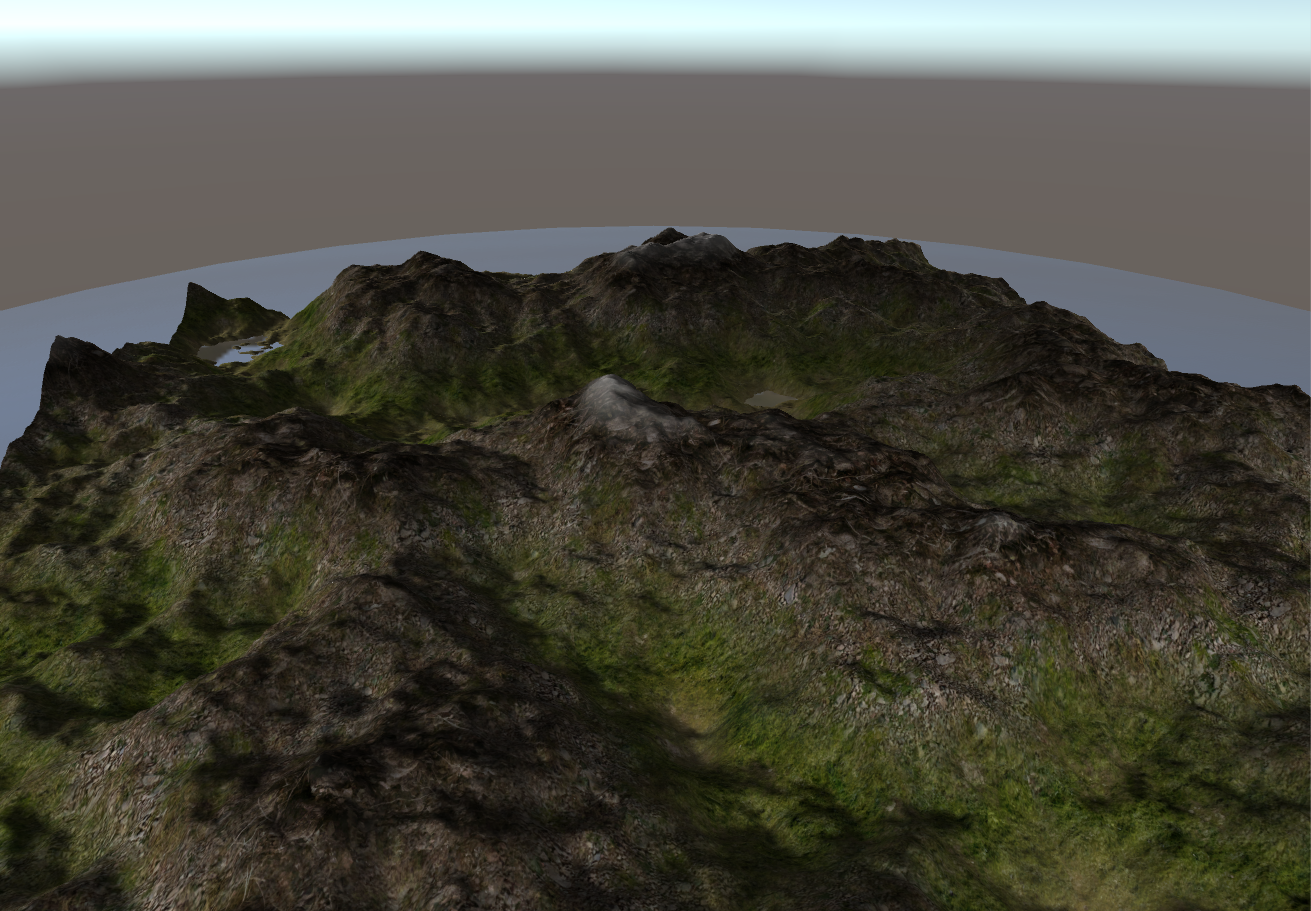
\includegraphics[width=\textwidth]{images/perlin_rendered.png}
	\caption{Texturierte Landschaft im Beispielprogramm die aus fraktalem Perlin-Noise entstanden ist.}\label{img.perlinRendered}
\end{figure}

\lstinputlisting[language=csh, title=Simple Fractal-Noise Implementierung C\#]{data/fractalNoise.cs}

\section{Flexibilität}\label{NoiseVariationen}
Die in \ref{eq.fractalnoise} beschriebene Funktion lässt sich beliebig erweitern und anpassen um bestimmte Effekte zu erzielen. Im folgenden sollen daher einige bekannte und für Landschaften passende Erweiterungen erläutert werden. Diese Auflistung ist nur als eine Auswahl zu verstehen. Es gibt noch zahlreiche weitere Implementierungen wie z.B. Convolution oder auch Sparse-Convolution-Noise\cite{texturingAndModeling}.

\subsection{Ridged-Noise}
In der Natur lassen sich in einigen Gebirgen sehr steile und gezahnte Kämme feststellen. Aufgrund der kontinuierlichen Natur einer Noise-Funktion sind die Kämme jedoch eher abgerundet. 
Um diesen Effekt aufzuheben wird der Betrag der Noise-Funktion von 1 abgezogen. 

\begin{equation} \label{eq.ridgedNoise}
ridged(\vec{x}) = \sum_{k=k_0}^{k_1}\frac{1}{r^{kH}}(1-\left|gnoise(r^k\vec{x})\right|).
\end{equation}

Anschaulich modelliert die Funktion nun Material aus einem Quader heraus anstatt die Landschaft auf eine Ebene rauf zu modellieren. Durch den Betrag verliert die Funktion außerdem ihre Stetigkeit in der ersten Ableitung, was zu einem abrupten Richtungswechseln der Höhenfunktion führt. An diesen Punkten entstehen nun, wie in \autoref{img.ridgedRendered}zu sehen, die erwünschten scharfen Kämme.

\begin{figure}[!hbtp]%
	\centering
	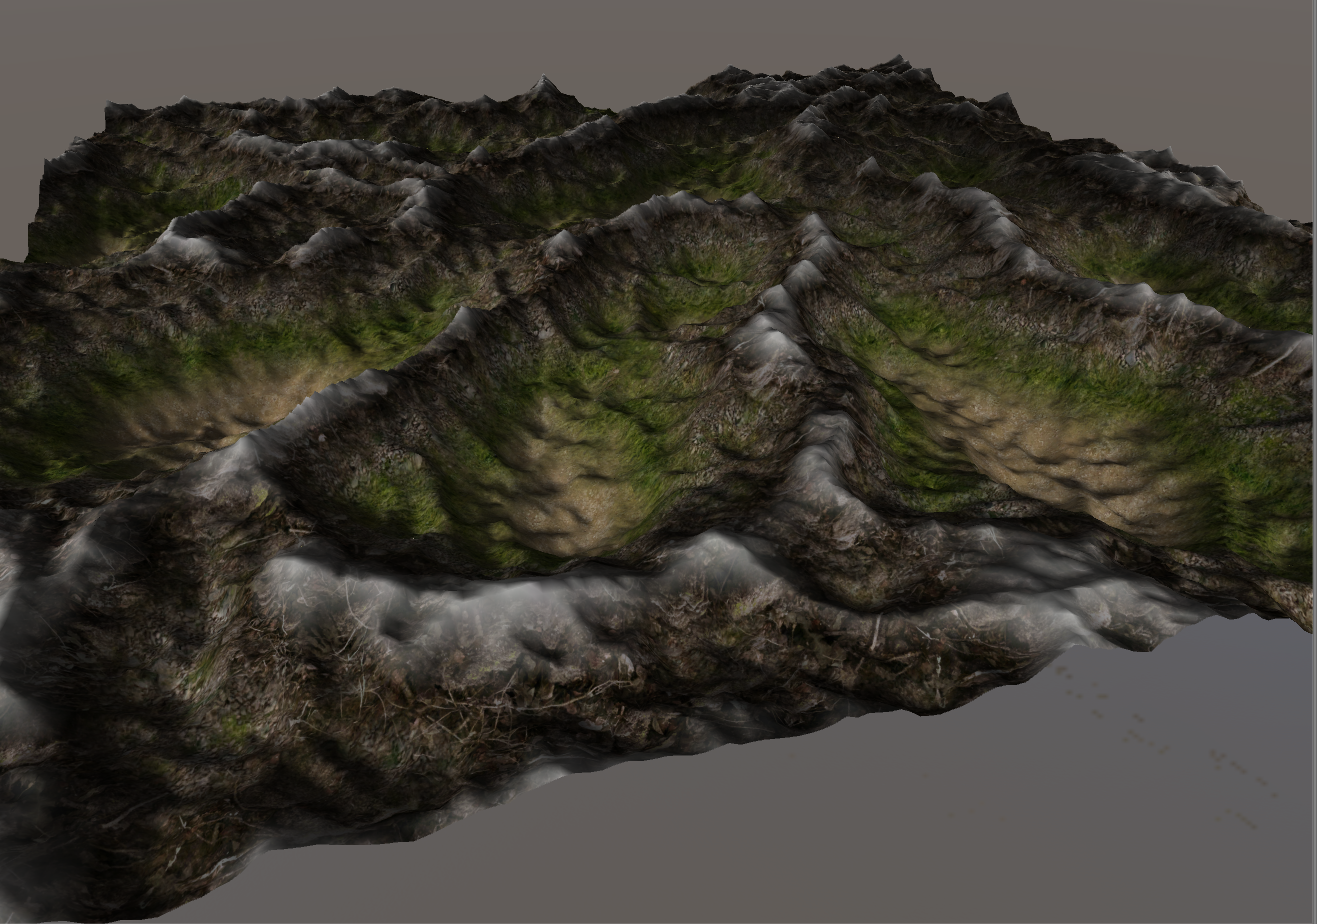
\includegraphics[width=\textwidth]{images/ridged_rendered.png}
	\caption{Texturierte Landschaft im Beispielprogramm die aus Ridged Noise entstanden ist}\label{img.ridgedRendered}
\end{figure}

\lstinputlisting[language=csh, title=Ridged-Noise Implementierung HLSL]{data/RidgedNoiseHLSL.hlsl}

\subsection{Multifraktal/heterogenes Terrain}
Wie auch in \ref{unisotrop} erwähnt kommen hohe Frequenzen momentan sowohl in den Tälern als auch auf den Bergen unserer Landschaft vor. Um diese homogenität zu verhindern wurde eine Noise Funktion entwickelt die durch Multiplikation der Oktaven zu einem Multifraktal führt\footnote{\cite{texturingAndModeling} p.440}. 

\begin{equation} \label{eq.multiNoise}
multi(\vec{x}) = \prod_{k=k_0}^{k_1}\frac{1}{r^{kH}}(gnoise(r^k\vec{x})+o).
\end{equation}

Es ist hierbei anzumerken, dass das Intervall des Ergebnisses dieser Rauschfunktion stark variiert. Um ein Ergebnis in einem konstanten Intervall zu verarbeiten muss im Nachhinein der höchste bzw. tiefste Punkt gesucht werden und entsprechend skaliert werden. Dadurch geht der Vorteil der parallelen Berechnung zur Echtzeit verloren. Eine andere Möglichkeit ist den Parameter $o$ entsprechend anzupassen um das Ergebnis in eine bestimmte Richtung zu beeinflussen. 
In \autoref{img.multiRendered} ist zu sehen, wie die tiefer gelegenen Gebiete deutlich weniger Anteile von hohen Frequenzen aufweisen und dadurch natürlicher wirken.

\begin{figure}
	\centering
	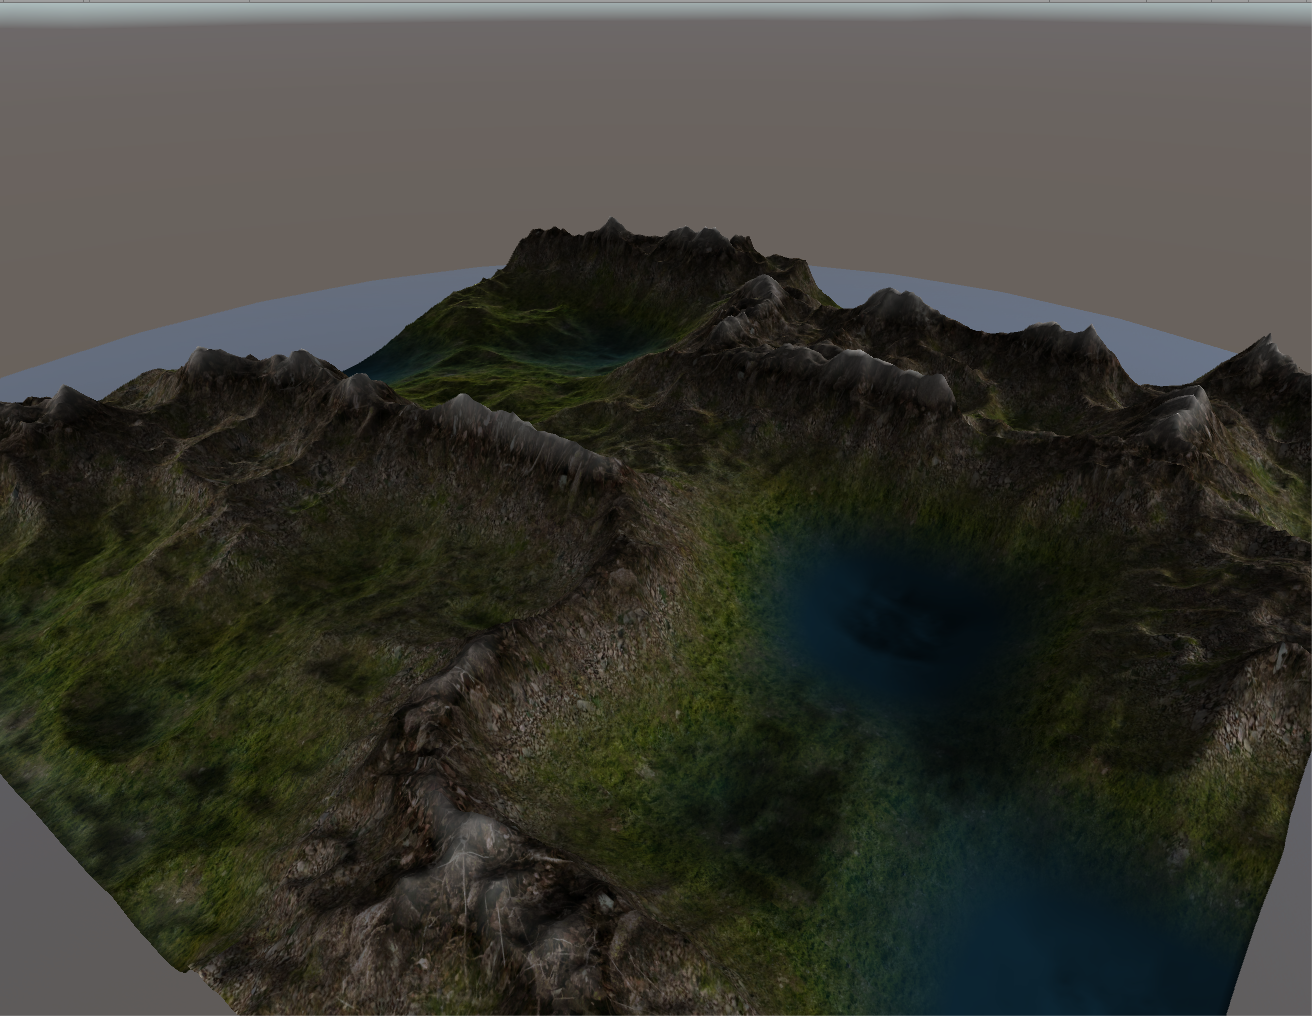
\includegraphics[width=\textwidth]{images/ridgedmulti_rendered.png}
	\caption{Texturierte Landschaft im Beispielprogramm die aus Ridged-Multifractal-Noise mit $o=0.2$ entstanden ist.}\label{img.multiRendered}
\end{figure}

\lstinputlisting[language=csh, title=Ridged-Multifractal Noise Implementierung HLSL]{data/RidgedMultiNoiseHLSL.hlsl}

\subsection{Hybrid-Multifractal}
Um das Problem des schwer zu bestimmenden Intervalls einer Multifraktalen Rauschfunktion zu umgehen und trotzdem ein heterogenes Terrain Ergebnis zu erzielen lassen sich die normale und die Multifraktale Rauschfunktion auch kombinieren. 
Die Heterogenität lässt sich dadurch erreichen, dass jede Oktave vor der Addition mit einem Gewicht multipliziert wird, welches das Produkt der vorherigen Oktaven ist. Dabei wird ein Faktor $w$ definiert, welcher das zu schnelle abfallen des Gewichtwertes bremst.


\begin{equation}
hybridnoise_{k1}(\vec{x}) = \sum_{k=k_0}^{k_1}s_k*octave_k
\end{equation}

\begin{equation}
s_i=\prod_{k=k_0}^{k_{i-1}}octave_k*w
\end{equation}

\begin{equation}
octave_k=\frac{1}{r^{kH}}gnoise(r^k\vec{x})
\end{equation}


In \autoref{img.hybridmultiRendered} ist zu sehen, dass hohe Frequenzen, wie beim Multifraktalem Rauschen, kaum noch Einfluss in den Tälern haben. 

\begin{figure}
	\centering
	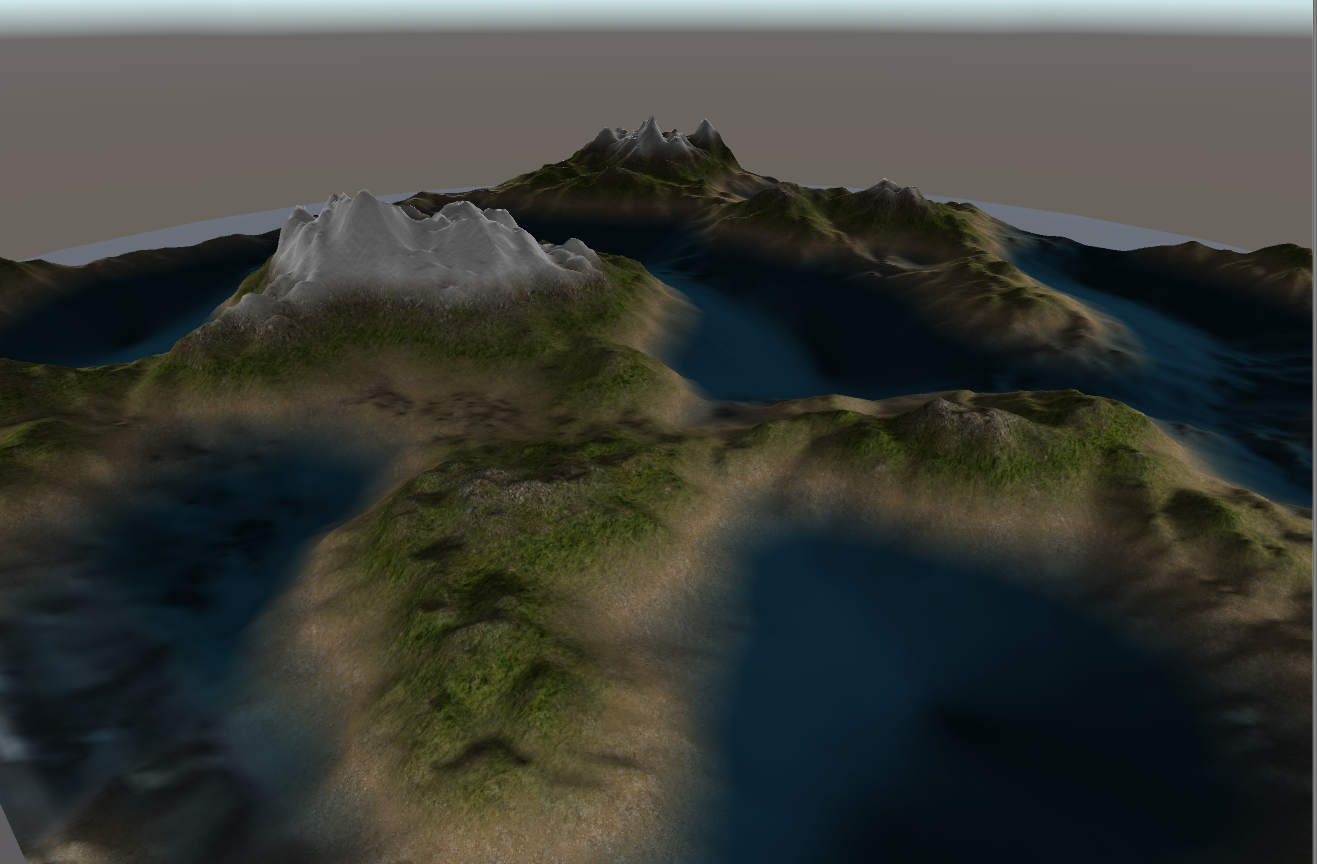
\includegraphics[width=\textwidth]{images/hybridmulti_rendered.png}
	\caption{Texturierte Landschaft im Beispielprogramm die aus Hybrid-Multifractal-Noise mit $o=0.5$ und $w=1.15$ entstanden ist.}\label{img.hybridmultiRendered}
\end{figure}


\lstinputlisting[language=csh, title=Hybrid-Multifractal Noise Implementierung HLSL]{data/HMFNoise.hlsl}


\subsection{Domain/Range Mapping}
Um die Rauschfunktion mit weiteren Effekten zu versehen lässt sich Domain bzw. Range Mapping anwendenden. 

Beim Domain Mapping handelt es sich um eine Modifikation der Definitionsmenge\footnote{englisch: Domain}. So wurde etwa in \autoref{img.domainwarpedRendered} der Eingangsvektor $\vec{x}$ proportional zur Höhe rotiert.

\begin{equation} \label{eq.domainrangemapping}
rangedomain(\vec{x}) = r\left( \sum_{k=k_0}^{k_1}\frac{1}{r^{kH}}(gnoise(d(r^k\vec{x})))\right)
\end{equation}

Range Mapping bezeichnet die nachträgliche Transformation des Ergebnisses der Rauschfunktion durch eine Funktion der Form $r(x): [-1-1]\to[-1-1]$.
Zum modellieren einer geeigneten Funktion $r$ bietet sich die von Ken Perlin in \cite{texturingAndModeling}\footnote{Seiten 339-400} vorgestellten
Bias und Gain Funktion an.


\subsubsection{Bias-Funktion}
Die Bias-Funktion ist im Intervall $[0-1]$ definiert und bei einem Funktionswert von $x=0.5$ seine Basis $b$ zurück. Durch die Veränderung dieser Basis lässt sich das Krümmungsverhalten der Funktion anpassen.

\begin{equation}
	bias_b(t)=t^{\frac{ln(b)}{ln(0.5)}}
\end{equation}

\begin{figure}[!hbtp]%
	
	
	\newcommand{\biasscale}{0.5}
	\centering
	\subcaptionbox{b=0.25}
	{
		\begin{tikzpicture}[scale=\biasscale]
		\begin{axis}
		[ 
		xlabel=$t$,
		ylabel={$bias_{0.25}(x)$},
		ymin=0,
		ymax=1,
		xmin=0,
		xmax=1,
		restrict x to domain=0:1
		] 
		
		\addplot[no markers, blue, smooth, domain = 0:1] {x^(ln(0.25)/ln(0.5))}; 
		\end{axis}
		\end{tikzpicture}
	}
	\subcaptionbox{b=0.5}
	{
		\begin{tikzpicture}[scale=\biasscale]
		\begin{axis}
		[ 
		xlabel=$t$,
		ylabel={$bias_{0.5}(x)$},
		ymin=0,
		ymax=1,
		xmin=0,
		xmax=1,
		restrict x to domain=0:1
		] 
		
		\addplot[no markers, blue, smooth, domain = 0:1] {x^(ln(0.5)/ln(0.5))}; 
		\end{axis}
		\end{tikzpicture}
	}
	\subcaptionbox{b=0.75}
	{
		\begin{tikzpicture}[scale=\biasscale]
		\begin{axis}
		[ 
		xlabel=$t$,
		ylabel={$bias_{0.75}(x)$},
		ymin=0,
		ymax=1,
		xmin=0,
		xmax=1,
		restrict x to domain=0:1
		] 
		
		\addplot[no markers, blue, smooth, domain = 0:1] {x^(ln(0.75)/ln(0.5))}; 
		\end{axis}
		\end{tikzpicture}
	}
	\caption{Bias-Funktion}
\end{figure}

\subsubsection{Gain-Funktion}
Im gleichen Intervall wie die Bias Funktion definiert, lässt sich mit Basis $g$ der Gain-Funktion kontrollieren, ob die Funktionswerte sich, wie in \autoref{img.gain} zu sehen, die meiste Zeit im Mittel oder an den Extremwerten(0 und 1) befinden.
\[
gain(t)= 
\begin{cases}
\frac{bias_{1-g}(2t)}{2},& \text{if } t>0.5\\
\frac{2-bias_{1-g}(2-2t)}{2},              & \text{if } t\leq0.5
\end{cases}
\]

\begin{figure}[!hbtp]%
	\centering
	\subcaptionbox{$g=0.25$\label{img.gain025}}
	{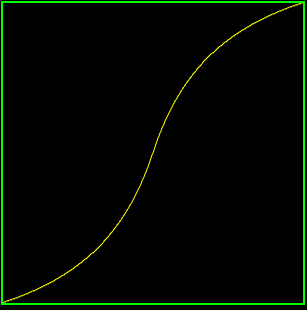
\includegraphics[width=0.24\textwidth]{images/gain025.png}}
	\subcaptionbox{$g=0.5$\label{img.gain05}} {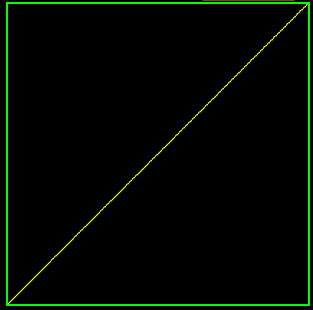
\includegraphics[width=0.24\textwidth]{images/gain05.png}}
	\subcaptionbox{$g=0.75$\label{img.gain075}} {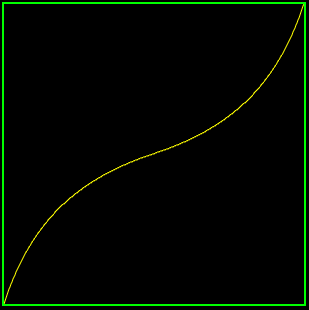
\includegraphics[width=0.24\textwidth]{images/gain075.png}}
	\subcaptionbox{$g=0.97$\label{img.gain097}} {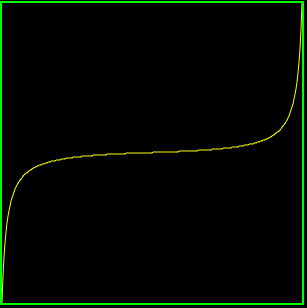
\includegraphics[width=0.24\textwidth]{images/gain097.png}}
	\caption{Verhalten der Gain-Funktion bei verschiedenen Werten für $g$. Bilder entnommen von: http://tinyurl.com/zgb6jaj}\label{img.gain}
\end{figure}


\begin{figure}[!hbtp]
	\centering
	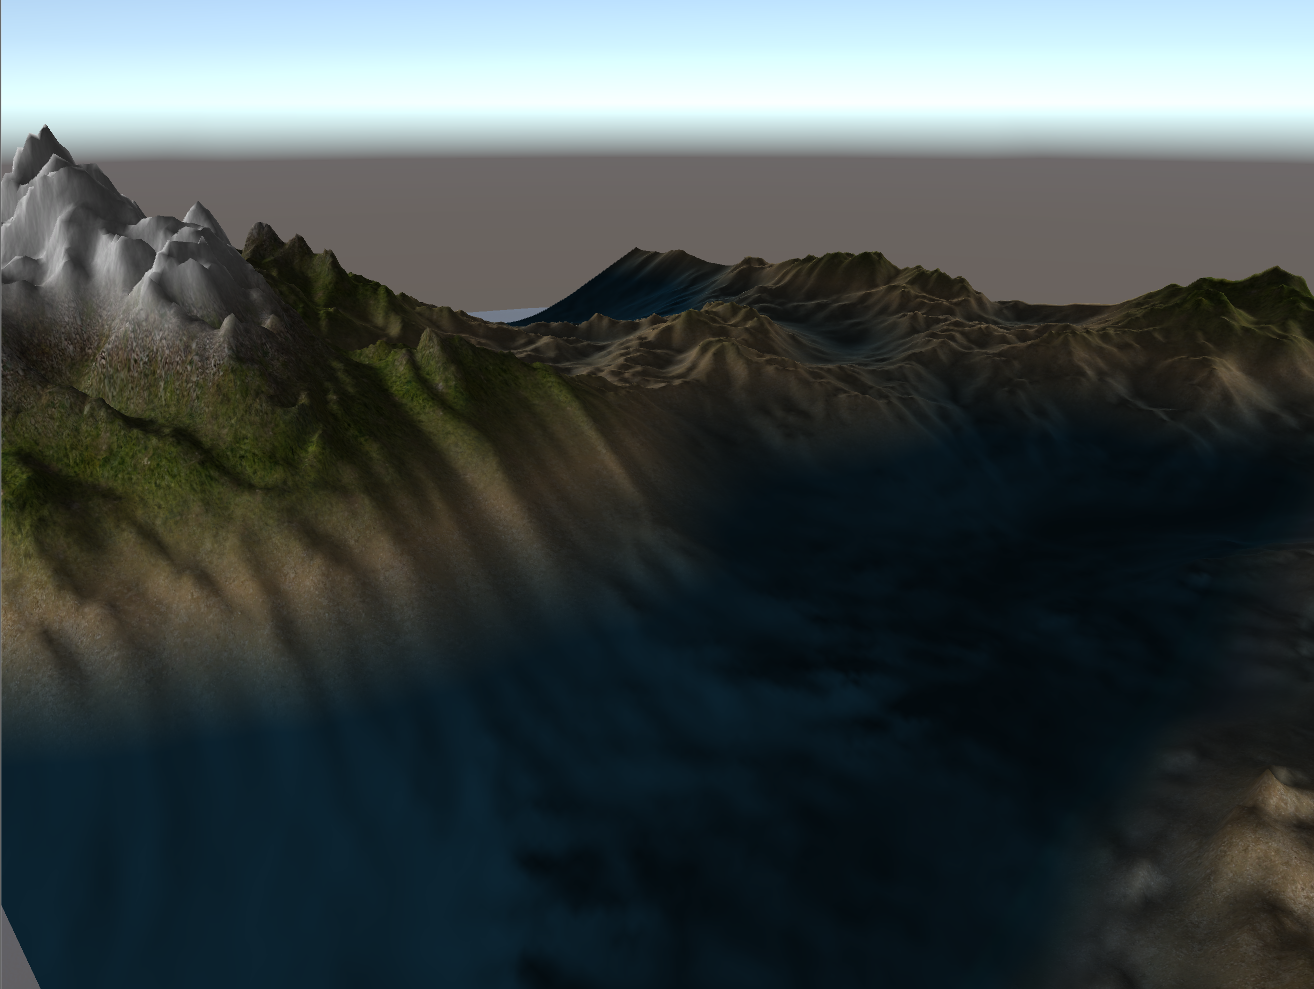
\includegraphics[width=\textwidth]{images/domainwarped_rendered.png}
	\caption{Texturierte Landschaft im Beispielprogramm die aus Domain Mapped Multifractal-Noise mit $o=0.48$ und $\alpha=20$ entstanden ist.}\label{img.domainwarpedRendered}
\end{figure}


\section{Bewertung im Rahmen der Fragestellung}
Das deterministische Verhalten von Rauschfunktionen erlaubt es einzig den Seed zur Erzeugung der Gitterwerte zu speichern. Durch die punktuelle Auswertung der Funktion lässt sich immer nur der Teil der Landschaft im Speicher halten, welcher gerade durch die virtuelle Kamera sichtbar ist. Eine Aufteilung des Geländes wie beim Diamond-Square Algorithmus vorgeschlagen\ref{Patches} ist nicht notwendig, wenn auch möglich um Ladezeiten zu vermeiden.








% Noch nicht bearbeitet
\chapter{weiteres Kapitel}\label{c.weitereskapitel}
In diesem Kapitel wird einiges gemacht\footnote{wobei einiges nicht vieles heißt, ich möchte hier also keine falschen Hoffnungen wecken.} Vor allem in \autoref{s.tiefer} wird einiges gezeigt, was noch nie jemand gesehen hat. Es lohnt sich also, dranzubleiben.

\section{eine Sektion}\label{s.einesektion}
Er hörte leise Schritte hinter sich. Das bedeutete nichts Gutes. Wer würde ihm schon folgen, spät in der Nacht und dazu noch in dieser engen Gasse mitten im übel beleumundeten Hafenviertel? Gerade jetzt, wo er das Ding seines Lebens gedreht hatte und mit der Beute verschwinden wollte! Hatte einer seiner zahllosen Kollegen dieselbe Idee gehabt, ihn beobachtet und abgewartet, um ihn nun um die Früchte seiner Arbeit zu erleichtern? \todotext{das muss ich noch verfeinern, weil ich erst zur Hälfte verstanden habe} Oder gehörten die Schritte hinter ihm zu einem der unzähligen Gesetzeshüter dieser Stadt, und die stählerne Acht um seine Handgelenke würde gleich zuschnappen? Er konnte die Aufforderung stehen zu bleiben schon hören. Gehetzt sah er sich um. Plötzlich erblickte er den schmalen Durchgang. Blitzartig drehte er sich nach rechts und verschwand zwischen den beiden Gebäuden. Beinahe wäre er dabei über den umgestürzten Mülleimer gefallen, der mitten im Weg lag. Er versuchte, sich in der Dunkelheit seinen Weg zu ertasten und erstarrte: Anscheinend gab es keinen anderen Ausweg aus diesem kleinen Hof als den Durchgang, durch den er gekommen war. Die Schritte wurden lauter und lauter, er sah eine dunkle Gestalt um die Ecke biegen. Fieberhaft irrten seine Augen durch die nächtliche Dunkelheit und suchten einen Ausweg. War jetzt wirklich alles vorbei, waren alle Mühe und alle Vorbereitungen umsonst? Er presste sich ganz eng an die Wand hinter ihm und hoffte, der Verfolger würde ihn übersehen, als plötzlich neben ihm mit kaum wahrnehmbarem Quietschen eine Tür im nächtlichen Wind hin und her schwang. Könnte dieses der flehentlich herbeigesehnte Ausweg aus seinem Dilemma sein? Langsam bewegte er sich auf die offene Tür zu, immer dicht an die Mauer gepresst. Würde diese Tür seine Rettung werden?


\bild{bild}{16cm}{Test-Bild mit langer Bildunterschrift}{Test-Bild}

Die \autoref{pythagoras}
\begin{equation}
a^2 + b^2 = c^2 \label{pythagoras}
\end{equation}
ist allseits bekannt und bedarf wohl keiner weiteren Erläuterung.

Auch nicht schlecht ist \autoref{img.bild}. Aber überhaupt keinen Sinn macht \autoref{tab.sinnlos}. Hieran sieht man den Vorteil des autoref-Befehls und das so Links erstellt werden.

\begin{table}[!hbt]\vspace{1ex}\centering\begin{tabular}{|l|l|}
\hline
Formen & Städte\\
\hline
\hline
Quadrat &  Bunkenstedt \\
\hline
Dreieck &  Laggenbeck\\
\hline
Kreis &  Peine\\
\hline
Raute & Wakaluba \\
\hline
\end{tabular}
\caption{\label{tab.sinnlos}eine sinnlose Tabelle}
\vspace{2ex}\end{table}


\subsection{jetzt geht es noch tiefer}\label{s.tiefer}

Er hörte leise Schritte hinter sich. Das bedeutete nichts Gutes. Wer würde ihm schon folgen, spät in der Nacht und dazu noch in dieser engen Gasse mitten im übel beleumundeten Hafenviertel? Gerade jetzt, wo er das Ding seines Lebens gedreht hatte und mit der Beute verschwinden wollte! Hatte einer seiner zahllosen Kollegen dieselbe Idee gehabt, ihn beobachtet und abgewartet, um ihn nun um die Früchte seiner Arbeit zu erleichtern? Oder gehörten die Schritte hinter ihm zu einem der unzähligen Gesetzeshüter dieser Stadt, und die stählerne Acht um seine Handgelenke würde gleich zuschnappen? Er konnte die Aufforderung stehen zu bleiben schon hören. Gehetzt sah er sich um. Plötzlich erblickte er den schmalen Durchgang. Blitzartig drehte er sich nach rechts und verschwand zwischen den beiden Gebäuden. Beinahe wäre er dabei über den umgestürzten Mülleimer gefallen, der mitten im Weg lag. Er versuchte, sich in der Dunkelheit seinen Weg zu ertasten und erstarrte: Anscheinend gab es keinen anderen Ausweg aus diesem kleinen Hof als den Durchgang, durch den er gekommen war. Die Schritte wurden lauter und lauter, er sah eine dunkle Gestalt um die Ecke biegen. Fieberhaft irrten seine Augen durch die nächtliche Dunkelheit und suchten einen Ausweg. War jetzt wirklich alles vorbei, waren alle Mühe und alle Vorbereitungen umsonst? Er presste sich ganz eng an die Wand hinter ihm und hoffte, der Verfolger würde ihn übersehen, als plötzlich neben ihm mit kaum wahrnehmbarem Quietschen eine Tür im nächtlichen Wind hin und her schwang. Könnte dieses der flehentlich herbeigesehnte Ausweg aus seinem Dilemma sein? Langsam bewegte er sich auf die offene Tür zu, immer dicht an die Mauer gepresst. Würde diese Tür seine Rettung werden?


\begin{figure}
\centering
\subcaptionbox{Ein Bild im PDF mit einer Größe von nur 1,1 kB\label{img.schwein1}} {
\includegraphics[width=0.49\textwidth]{images/schwein1}}
\subcaptionbox{Das gleiche Bild als optimierte PNG-Datei mit einer Größe von 8,9 kB\label{img.schwein2}}
{
\includegraphics[width=0.49\textwidth]{images/schwein2}}
\caption{Zwei Bilder werden mit dem \LaTeX-Paket subcaption nebeneinander angezeigt}\label{img.subcaption}
\end{figure}

Auch können Bilder in Bildern direkt angesprochen werden: \autoref{img.schwein1} und  \autoref{img.schwein2}.


Er hörte leise Schritte hinter sich. Das bedeutete nichts Gutes. Wer würde ihm schon folgen, spät in der Nacht und dazu noch in dieser engen Gasse mitten im übel beleumundeten Hafenviertel? Gerade jetzt, wo er das Ding seines Lebens gedreht hatte und mit der Beute verschwinden wollte! Hatte einer seiner zahllosen Kollegen dieselbe Idee gehabt, ihn beobachtet und abgewartet, um ihn nun um die Früchte seiner Arbeit zu erleichtern? Oder gehörten die Schritte hinter ihm zu einem der unzähligen Gesetzeshüter dieser Stadt, und die stählerne Acht um seine Handgelenke würde gleich zuschnappen? Er konnte die Aufforderung stehen zu bleiben schon hören. Gehetzt sah er sich um.

\begin{itemize}
\item Erstens ist das soundso,

\item dann darf man natürlich nicht vergessen und

\item das ist auch noch wichtig.
\end{itemize}


Plötzlich erblickte er den schmalen Durchgang. Blitzartig drehte er sich nach rechts und verschwand zwischen den beiden Gebäuden. Beinahe wäre er dabei über den umgestürzten Mülleimer gefallen, der mitten im Weg lag. Er versuchte, sich in der Dunkelheit seinen Weg zu ertasten und erstarrte: Anscheinend gab es keinen anderen Ausweg aus diesem kleinen Hof als den Durchgang, durch den er gekommen war. Die Schritte wurden lauter und lauter, er sah eine dunkle Gestalt um die Ecke biegen. Fieberhaft irrten seine Augen durch die nächtliche Dunkelheit und suchten einen Ausweg. War jetzt wirklich alles vorbei, waren alle Mühe und alle Vorbereitungen umsonst? Er presste sich ganz eng an die Wand hinter ihm und hoffte, der Verfolger würde ihn übersehen, als plötzlich neben ihm mit kaum wahrnehmbarem Quietschen eine Tür im nächtlichen Wind hin und her schwang. Könnte dieses der flehentlich herbeigesehnte Ausweg aus seinem Dilemma sein? Langsam bewegte er sich auf die offene Tür zu, immer dicht an die Mauer gepresst. Würde diese Tür seine Rettung werden?






Komplexe Tabellen sind nicht sehr einfach:

\begin{table}[!hbt]\vspace{1ex}\centering
\begin{tabular}{|ll||l|l|l|l|}\hline
\multicolumn{2}{|c||}{}&\multicolumn{4}{c|}{ dies} \\
\multicolumn{2}{|c||}{}& von dort  & und dort & über hier & zu Los \\\hline\hline
\multirow{3}*{\rotatebox{90}{das}} & hier &  bla  & bla  & bla  & bla \\\cline{2-6}
& dort & bla  & bla & bla  & bla  \\\cline{2-6}
& da &  bla  & bla & bla & bla \\\hline
\end{tabular}
\caption[eine kompliziertere Tabelle]{eine kompliziertere Tabelle mit viel Beschreibungstext, der aber nicht im Tabellenverzeichnis auftauschen soll}
\vspace{2ex}\end{table}


Er hörte leise Schritte hinter sich. Das bedeutete nichts Gutes. Wer würde ihm schon folgen, spät in der Nacht und dazu noch in dieser engen Gasse mitten im übel beleumundeten Hafenviertel? Gerade jetzt, wo er das Ding seines Lebens gedreht hatte und mit der Beute verschwinden wollte! Hatte einer seiner zahllosen Kollegen dieselbe Idee gehabt, ihn beobachtet und abgewartet, um ihn nun um die Früchte seiner Arbeit zu erleichtern? Oder gehörten die Schritte hinter ihm zu einem der unzähligen Gesetzeshüter dieser Stadt, und die stählerne Acht um seine Handgelenke würde gleich zuschnappen? Er konnte die Aufforderung stehen zu bleiben schon hören. Gehetzt sah er sich um. Plötzlich erblickte er den schmalen Durchgang. Blitzartig drehte er sich nach rechts und verschwand zwischen den beiden Gebäuden. Beinahe wäre er dabei über den umgestürzten Mülleimer gefallen, der mitten im Weg lag. Er versuchte, sich in der Dunkelheit seinen Weg zu ertasten und erstarrte: Anscheinend gab es keinen anderen Ausweg aus diesem kleinen Hof als den Durchgang, durch den er gekommen war. Die Schritte wurden lauter und lauter, er sah eine dunkle Gestalt um die Ecke biegen. Fieberhaft irrten seine Augen durch die nächtliche Dunkelheit und suchten einen Ausweg. War jetzt wirklich alles vorbei, waren alle Mühe und alle Vorbereitungen umsonst? Er presste sich ganz eng an die Wand hinter ihm und hoffte, der Verfolger würde ihn übersehen, als plötzlich neben ihm mit kaum wahrnehmbarem Quietschen eine Tür im nächtlichen Wind hin und her schwang. Könnte dieses der flehentlich herbeigesehnte Ausweg aus seinem Dilemma sein? Langsam bewegte er sich auf die offene Tür zu, immer dicht an die Mauer gepresst. Würde diese Tür seine Rettung werden?

\chapter{Zusammenfassung}\label{c.zusammenfassung}

Er hörte leise Schritte hinter sich. Das bedeutete nichts Gutes. Wer würde ihm schon folgen, spät in der Nacht und dazu noch in dieser engen Gasse mitten im übel beleumundeten Hafenviertel? Gerade jetzt, wo er das Ding seines Lebens gedreht hatte und mit der Beute verschwinden wollte! Hatte einer seiner zahllosen Kollegen dieselbe Idee gehabt, ihn beobachtet und abgewartet, um ihn nun um die Früchte seiner Arbeit zu erleichtern? Oder gehörten die Schritte hinter ihm zu einem der unzähligen Gesetzeshüter dieser Stadt, und die stählerne Acht um seine Handgelenke würde gleich zuschnappen? Er konnte die Aufforderung stehen zu bleiben schon hören. Gehetzt sah er sich um. Plötzlich erblickte er den schmalen Durchgang. Blitzartig drehte er sich nach rechts und verschwand zwischen den beiden Gebäuden. Beinahe wäre er dabei über den umgestürzten Mülleimer gefallen, der mitten im Weg lag. Er versuchte, sich in der Dunkelheit seinen Weg zu ertasten und erstarrte: Anscheinend gab es keinen anderen Ausweg aus diesem kleinen Hof als den Durchgang, durch den er gekommen war. Die Schritte wurden lauter und lauter, er sah eine dunkle Gestalt um die Ecke biegen. Fieberhaft irrten seine Augen durch die nächtliche Dunkelheit und suchten einen Ausweg. War jetzt wirklich alles vorbei, waren alle Mühe und alle Vorbereitungen umsonst? Er presste sich ganz eng an die Wand hinter ihm und hoffte, der Verfolger würde ihn übersehen, als plötzlich neben ihm mit kaum wahrnehmbarem Quietschen eine Tür im nächtlichen Wind hin und her schwang. Könnte dieses der flehentlich herbeigesehnte Ausweg aus seinem Dilemma sein? Langsam bewegte er sich auf die offene Tür zu, immer dicht an die Mauer gepresst. Würde diese Tür seine Rettung werden?


% Anhang
\begin{landscape}\begin{multicols}{2}
\appendix
\chapter{Anhang}
\section{Quelltexte}
\subsubsection*{cpu.c aus Linux 2.6.16}\label{s.cpu}\lstinputlisting[language=C]{code/cpu.c}
\end{multicols}\end{landscape}


\bibliographystyle{alphadin_martin}
\bibliography{bibliographie}


\chapter*{Erklärung}

Hiermit versichere ich, dass ich die vorliegende Arbeit selbstständig verfasst und keine anderen als die angegebenen Quellen und Hilfsmittel benutzt habe, dass alle Stellen der Arbeit, die wörtlich oder sinngemäß aus anderen Quellen übernommen wurden, als solche kenntlich gemacht und dass die Arbeit in gleicher oder ähnlicher Form noch keiner Prüfungsbehörde vorgelegt wurde.

\vspace{3cm}
Ort, Datum \hspace{5cm} Unterschrift\\

\end{document}